\documentclass[12pt, twoside]{article}
\usepackage[letterpaper, margin=1in, headsep=0.5in]{geometry}
\usepackage[english]{babel}
\usepackage[utf8]{inputenc}
\usepackage{amsmath}
\usepackage{amsfonts}
\usepackage{amssymb}
\usepackage{tikz}
%\usetikzlibrary{quotes, angles}

\usepackage{graphicx}
\usepackage{enumitem}
\usepackage{multicol}

\usepackage{fancyhdr}
\pagestyle{fancy}
\fancyhf{}
\renewcommand{\headrulewidth}{0pt} % disable the underline of the header

\fancyhead[RE]{\thepage}
\fancyhead[RO]{\thepage \\ Name: \hspace{3cm}}
\fancyhead[L]{BECA / Dr. Huson / Geometry\\* 1 February 2019}

\begin{document}
\subsubsection*{7-4 Do Now: Graphing linear equations}
  \begin{enumerate}

\item Graph and label the two equations. Mark their intersection as an ordered pair.

  \begin{multicols}{2}
    $y = -2x+3$ \\
    $2x-4y = 8$
  \end{multicols}
  Are the lines parallel, perpendicular, or neither? Justify your answer.
  \vspace{1.5cm}

  \begin{center} %4 quadrant regents grid w T-Chart
  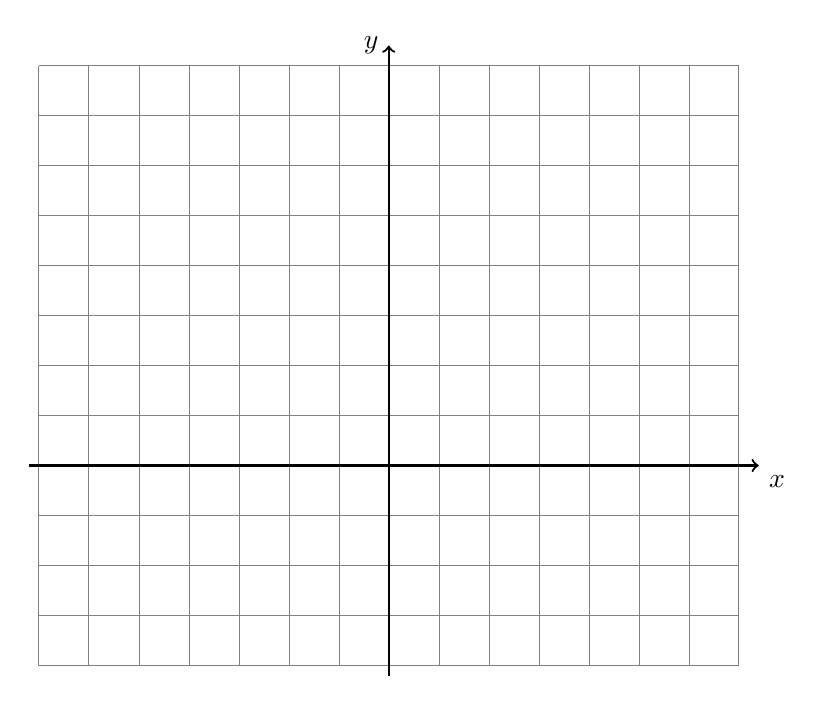
\begin{tikzpicture}[scale=.635]
    \draw [help lines] (-7,-4) grid (7,8);
    \draw [thick, ->] (-7.2,0) -- (7.4,0) node [below right] {$x$};
    \draw [thick, ->] (0,-4.2)--(0,8.4) node [left] {$y$};
  \end{tikzpicture}
  \end{center}


    \item A translation of $x \rightarrow x+2, y \rightarrow y-4$ maps $\overline{AB} \rightarrow \overline{CD}$, with $A(-2,0)$ and $B(0,5)$. Find the slopes and $y$-intercepts of $\overleftrightarrow{AB}$ and $\overleftrightarrow{CD}$, and hence write down the equations of the two lines.

\newpage

\item On the graph, draw $\triangle ABC$ with vertices A(-2, 1), B(9,-1), C(1, 5). Prove that $\triangle ABC$ is a right triangle by showing $\overline{AC} \perp \overline{BC}$. Complete the concluding statements given.\\[1cm]
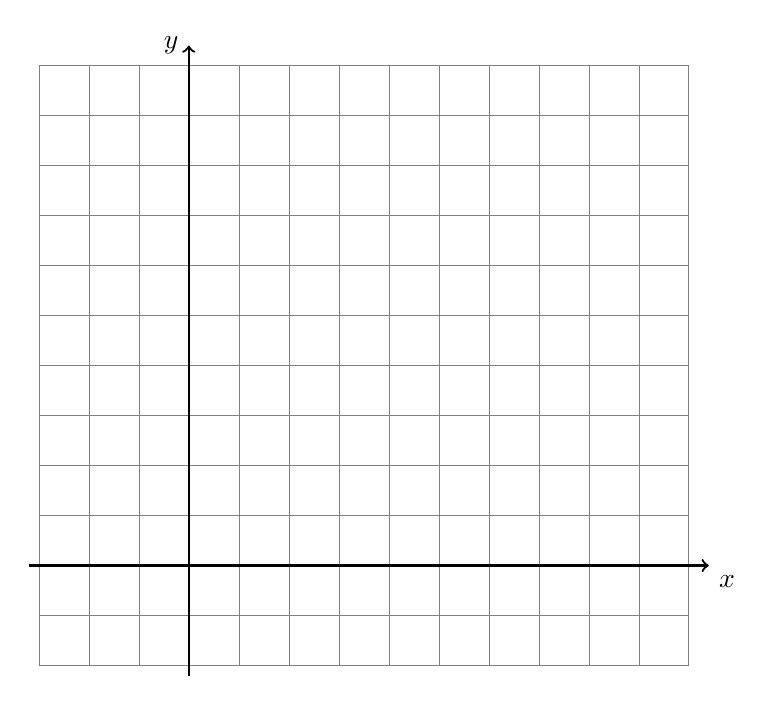
\begin{tikzpicture}[scale=.635]
  \draw [help lines] (-3,-2) grid (10,10);
  \draw [thick, ->] (-3.2,0) -- (10.4,0) node [below right] {$x$};
  \draw [thick, ->] (0,-2.2)--(0,10.4) node [left] {$y$};
\end{tikzpicture}
\vspace{8cm}

Segment $\overline{AC}$ and segment $\rule{1.5cm}{0.15mm}$ are perpendicular so $\angle C$ is a $\rule{1.5cm}{0.15mm}$ angle.\\[0.5cm]
Angle $\rule{1.5cm}{0.15mm}$ is a right angle so $\triangle ABC$ is a right triangle.

  \end{enumerate}
  \newpage
  \setcounter{page}{1}

\subsubsection*{7-4 Homework: Quadratic functions}
Show your work. For graphs, use a pencil and straight edge.
  \begin{enumerate}

\item Graph and label each function. Mark the vertices as ordered pairs and the $x$- and $y$-intercepts with their values.
        \vspace{0.25cm}
        \begin{multicols}{2}
          $f(x)=x^2$\\
          $g(x)=(x+4)^2-1$
        \end{multicols}
        What transformation maps $f$ onto $g$?
        \vspace{2.25cm}

    \begin{center} %4 quadrant regents grid w T-Chart
    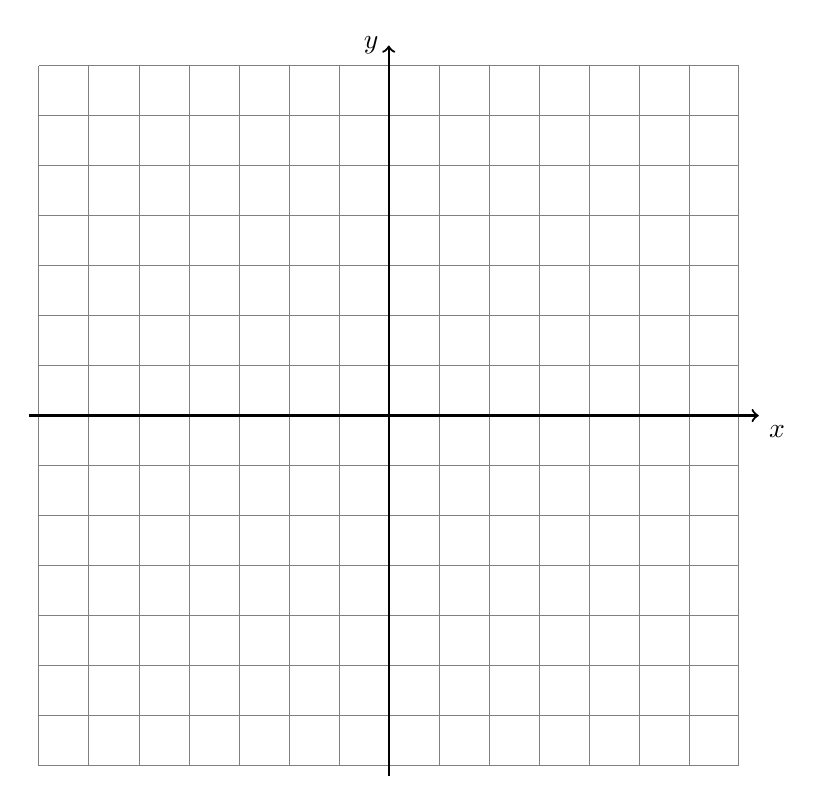
\begin{tikzpicture}[scale=.635]
      \draw [help lines] (-7,-7) grid (7,7);
      \draw [thick, ->] (-7.2,0) -- (7.4,0) node [below right] {$x$};
      \draw [thick, ->] (0,-7.2)--(0,7.4) node [left] {$y$};
    \end{tikzpicture}
    \end{center}


    In the following two problems, solve for the value of $x$.
    \begin{multicols}{2}
    \item   $\frac{3}{4}(x+5)=5$ \vspace{3cm}
    \item   $\frac{1}{3}(6-3x)=-7$ \vspace{3cm}
    \end{multicols}

\newpage

\item Given $f(x)=x^2-7x+3$. Simplify $f(0)$. \vspace{2cm}
\item Given $g(x)=\frac{2}{5} x-1$. Solve for $x$ such that for $g(x)=3$. \vspace{2.5cm}
\item Solve $x^2-6x-7=0$. \vspace{3cm}


\item On the graph, draw $\triangle ABC$ with vertices A(0, 2), B(6,-1), C(-2, -2). Prove that $\triangle ABC$ is a right triangle by showing $\overline{AC} \perp \overline{AB}$. \\[0.5cm]
Be sure to include a concluding statement.\\[1cm]
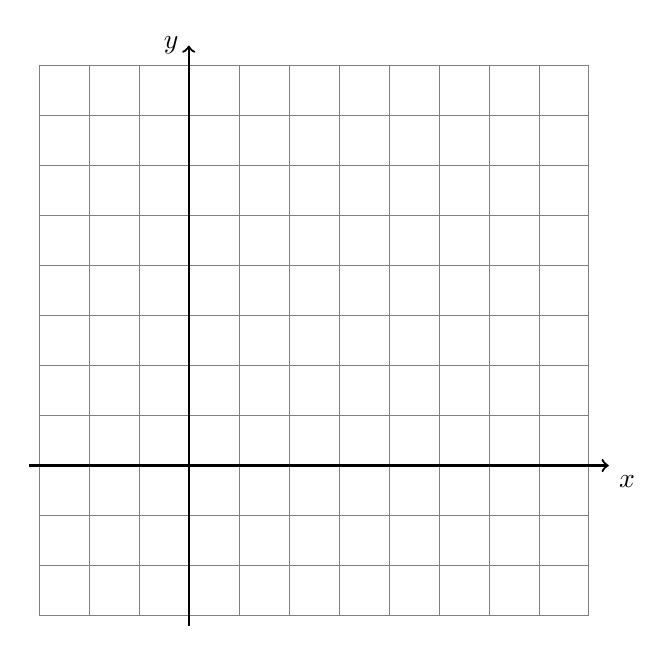
\begin{tikzpicture}[scale=.635]
  \draw [help lines] (-3,-3) grid (8,8);
  \draw [thick, ->] (-3.2,0) -- (8.4,0) node [below right] {$x$};
  \draw [thick, ->] (0,-3.2)--(0,8.4) node [left] {$y$};
\end{tikzpicture}

\end{enumerate}

\end{document}
